\documentclass[]{article}
\usepackage{lmodern}
\usepackage{amssymb,amsmath}
\usepackage{ifxetex,ifluatex}
\usepackage{fixltx2e} % provides \textsubscript
\ifnum 0\ifxetex 1\fi\ifluatex 1\fi=0 % if pdftex
  \usepackage[T1]{fontenc}
  \usepackage[utf8]{inputenc}
\else % if luatex or xelatex
  \ifxetex
    \usepackage{mathspec}
  \else
    \usepackage{fontspec}
  \fi
  \defaultfontfeatures{Ligatures=TeX,Scale=MatchLowercase}
\fi
% use upquote if available, for straight quotes in verbatim environments
\IfFileExists{upquote.sty}{\usepackage{upquote}}{}
% use microtype if available
\IfFileExists{microtype.sty}{%
\usepackage{microtype}
\UseMicrotypeSet[protrusion]{basicmath} % disable protrusion for tt fonts
}{}
\usepackage[margin=1in]{geometry}
\usepackage{hyperref}
\PassOptionsToPackage{usenames,dvipsnames}{color} % color is loaded by hyperref
\hypersetup{unicode=true,
            pdftitle={Design and Results for Wine Tasting Experiment},
            colorlinks=true,
            linkcolor=Maroon,
            citecolor=Blue,
            urlcolor=blue,
            breaklinks=true}
\urlstyle{same}  % don't use monospace font for urls
\usepackage{color}
\usepackage{fancyvrb}
\newcommand{\VerbBar}{|}
\newcommand{\VERB}{\Verb[commandchars=\\\{\}]}
\DefineVerbatimEnvironment{Highlighting}{Verbatim}{commandchars=\\\{\}}
% Add ',fontsize=\small' for more characters per line
\usepackage{framed}
\definecolor{shadecolor}{RGB}{248,248,248}
\newenvironment{Shaded}{\begin{snugshade}}{\end{snugshade}}
\newcommand{\AlertTok}[1]{\textcolor[rgb]{0.94,0.16,0.16}{#1}}
\newcommand{\AnnotationTok}[1]{\textcolor[rgb]{0.56,0.35,0.01}{\textbf{\textit{#1}}}}
\newcommand{\AttributeTok}[1]{\textcolor[rgb]{0.77,0.63,0.00}{#1}}
\newcommand{\BaseNTok}[1]{\textcolor[rgb]{0.00,0.00,0.81}{#1}}
\newcommand{\BuiltInTok}[1]{#1}
\newcommand{\CharTok}[1]{\textcolor[rgb]{0.31,0.60,0.02}{#1}}
\newcommand{\CommentTok}[1]{\textcolor[rgb]{0.56,0.35,0.01}{\textit{#1}}}
\newcommand{\CommentVarTok}[1]{\textcolor[rgb]{0.56,0.35,0.01}{\textbf{\textit{#1}}}}
\newcommand{\ConstantTok}[1]{\textcolor[rgb]{0.00,0.00,0.00}{#1}}
\newcommand{\ControlFlowTok}[1]{\textcolor[rgb]{0.13,0.29,0.53}{\textbf{#1}}}
\newcommand{\DataTypeTok}[1]{\textcolor[rgb]{0.13,0.29,0.53}{#1}}
\newcommand{\DecValTok}[1]{\textcolor[rgb]{0.00,0.00,0.81}{#1}}
\newcommand{\DocumentationTok}[1]{\textcolor[rgb]{0.56,0.35,0.01}{\textbf{\textit{#1}}}}
\newcommand{\ErrorTok}[1]{\textcolor[rgb]{0.64,0.00,0.00}{\textbf{#1}}}
\newcommand{\ExtensionTok}[1]{#1}
\newcommand{\FloatTok}[1]{\textcolor[rgb]{0.00,0.00,0.81}{#1}}
\newcommand{\FunctionTok}[1]{\textcolor[rgb]{0.00,0.00,0.00}{#1}}
\newcommand{\ImportTok}[1]{#1}
\newcommand{\InformationTok}[1]{\textcolor[rgb]{0.56,0.35,0.01}{\textbf{\textit{#1}}}}
\newcommand{\KeywordTok}[1]{\textcolor[rgb]{0.13,0.29,0.53}{\textbf{#1}}}
\newcommand{\NormalTok}[1]{#1}
\newcommand{\OperatorTok}[1]{\textcolor[rgb]{0.81,0.36,0.00}{\textbf{#1}}}
\newcommand{\OtherTok}[1]{\textcolor[rgb]{0.56,0.35,0.01}{#1}}
\newcommand{\PreprocessorTok}[1]{\textcolor[rgb]{0.56,0.35,0.01}{\textit{#1}}}
\newcommand{\RegionMarkerTok}[1]{#1}
\newcommand{\SpecialCharTok}[1]{\textcolor[rgb]{0.00,0.00,0.00}{#1}}
\newcommand{\SpecialStringTok}[1]{\textcolor[rgb]{0.31,0.60,0.02}{#1}}
\newcommand{\StringTok}[1]{\textcolor[rgb]{0.31,0.60,0.02}{#1}}
\newcommand{\VariableTok}[1]{\textcolor[rgb]{0.00,0.00,0.00}{#1}}
\newcommand{\VerbatimStringTok}[1]{\textcolor[rgb]{0.31,0.60,0.02}{#1}}
\newcommand{\WarningTok}[1]{\textcolor[rgb]{0.56,0.35,0.01}{\textbf{\textit{#1}}}}
\usepackage{graphicx,grffile}
\makeatletter
\def\maxwidth{\ifdim\Gin@nat@width>\linewidth\linewidth\else\Gin@nat@width\fi}
\def\maxheight{\ifdim\Gin@nat@height>\textheight\textheight\else\Gin@nat@height\fi}
\makeatother
% Scale images if necessary, so that they will not overflow the page
% margins by default, and it is still possible to overwrite the defaults
% using explicit options in \includegraphics[width, height, ...]{}
\setkeys{Gin}{width=\maxwidth,height=\maxheight,keepaspectratio}
\IfFileExists{parskip.sty}{%
\usepackage{parskip}
}{% else
\setlength{\parindent}{0pt}
\setlength{\parskip}{6pt plus 2pt minus 1pt}
}
\setlength{\emergencystretch}{3em}  % prevent overfull lines
\providecommand{\tightlist}{%
  \setlength{\itemsep}{0pt}\setlength{\parskip}{0pt}}
\setcounter{secnumdepth}{0}
% Redefines (sub)paragraphs to behave more like sections
\ifx\paragraph\undefined\else
\let\oldparagraph\paragraph
\renewcommand{\paragraph}[1]{\oldparagraph{#1}\mbox{}}
\fi
\ifx\subparagraph\undefined\else
\let\oldsubparagraph\subparagraph
\renewcommand{\subparagraph}[1]{\oldsubparagraph{#1}\mbox{}}
\fi

%%% Use protect on footnotes to avoid problems with footnotes in titles
\let\rmarkdownfootnote\footnote%
\def\footnote{\protect\rmarkdownfootnote}

%%% Change title format to be more compact
\usepackage{titling}

% Create subtitle command for use in maketitle
\newcommand{\subtitle}[1]{
  \posttitle{
    \begin{center}\large#1\end{center}
    }
}

\setlength{\droptitle}{-2em}

  \title{Design and Results for Wine Tasting Experiment}
    \pretitle{\vspace{\droptitle}\centering\huge}
  \posttitle{\par}
    \author{}
    \preauthor{}\postauthor{}
    \date{}
    \predate{}\postdate{}
  

\begin{document}
\maketitle

\begin{Shaded}
\begin{Highlighting}[]
\CommentTok{## Get the data}
\NormalTok{data <-}\StringTok{ }\KeywordTok{read.csv}\NormalTok{(}\DataTypeTok{file =} \StringTok{"chehalem_winery.csv"}\NormalTok{, }\DataTypeTok{header =}\NormalTok{ T)}
\NormalTok{A <-}\StringTok{ }\KeywordTok{factor}\NormalTok{(data}\OperatorTok{$}\NormalTok{A, }\DataTypeTok{levels =} \KeywordTok{c}\NormalTok{(}\OperatorTok{-}\DecValTok{1}\NormalTok{,}\DecValTok{1}\NormalTok{), }\DataTypeTok{labels =} \KeywordTok{c}\NormalTok{(}\StringTok{"Pommard"}\NormalTok{, }\StringTok{"Wadenswil"}\NormalTok{))}
\NormalTok{B <-}\StringTok{ }\KeywordTok{factor}\NormalTok{(data}\OperatorTok{$}\NormalTok{B, }\DataTypeTok{levels =} \KeywordTok{c}\NormalTok{(}\OperatorTok{-}\DecValTok{1}\NormalTok{,}\DecValTok{1}\NormalTok{), }\DataTypeTok{labels =} \KeywordTok{c}\NormalTok{(}\StringTok{"Allier"}\NormalTok{, }\StringTok{"Troncais"}\NormalTok{))}
\NormalTok{C <-}\StringTok{ }\KeywordTok{factor}\NormalTok{(data}\OperatorTok{$}\NormalTok{C, }\DataTypeTok{levels =} \KeywordTok{c}\NormalTok{(}\OperatorTok{-}\DecValTok{1}\NormalTok{,}\DecValTok{1}\NormalTok{), }\DataTypeTok{labels =} \KeywordTok{c}\NormalTok{(}\StringTok{"Old"}\NormalTok{, }\StringTok{"New"}\NormalTok{))}
\NormalTok{D <-}\StringTok{ }\KeywordTok{factor}\NormalTok{(data}\OperatorTok{$}\NormalTok{D, }\DataTypeTok{levels =} \KeywordTok{c}\NormalTok{(}\OperatorTok{-}\DecValTok{1}\NormalTok{,}\DecValTok{1}\NormalTok{), }\DataTypeTok{labels =} \KeywordTok{c}\NormalTok{(}\StringTok{"Champagne"}\NormalTok{, }\StringTok{"Montrachet"}\NormalTok{))}
\NormalTok{E <-}\StringTok{ }\KeywordTok{factor}\NormalTok{(data}\OperatorTok{$}\NormalTok{E, }\DataTypeTok{levels =} \KeywordTok{c}\NormalTok{(}\OperatorTok{-}\DecValTok{1}\NormalTok{,}\DecValTok{1}\NormalTok{), }\DataTypeTok{labels =} \KeywordTok{c}\NormalTok{(}\StringTok{"None"}\NormalTok{, }\StringTok{"All"}\NormalTok{))}
\NormalTok{F <-}\StringTok{ }\KeywordTok{factor}\NormalTok{(data}\OperatorTok{$}\NormalTok{F, }\DataTypeTok{levels =} \KeywordTok{c}\NormalTok{(}\OperatorTok{-}\DecValTok{1}\NormalTok{,}\DecValTok{1}\NormalTok{), }\DataTypeTok{labels =} \KeywordTok{c}\NormalTok{(}\StringTok{"Light"}\NormalTok{, }\StringTok{"Medium"}\NormalTok{))}
\NormalTok{G <-}\StringTok{ }\KeywordTok{factor}\NormalTok{(data}\OperatorTok{$}\NormalTok{G, }\DataTypeTok{levels =} \KeywordTok{c}\NormalTok{(}\OperatorTok{-}\DecValTok{1}\NormalTok{,}\DecValTok{1}\NormalTok{), }\DataTypeTok{labels =} \KeywordTok{c}\NormalTok{(}\StringTok{"None"}\NormalTok{, }\StringTok{"10%"}\NormalTok{))}
\NormalTok{H <-}\StringTok{ }\KeywordTok{factor}\NormalTok{(data}\OperatorTok{$}\NormalTok{H, }\DataTypeTok{levels =} \KeywordTok{c}\NormalTok{(}\OperatorTok{-}\DecValTok{1}\NormalTok{,}\DecValTok{1}\NormalTok{), }\DataTypeTok{labels =} \KeywordTok{c}\NormalTok{(}\StringTok{"Low"}\NormalTok{, }\StringTok{"High"}\NormalTok{))}
\NormalTok{y <-}\StringTok{ }\NormalTok{data}\OperatorTok{$}\NormalTok{y}
\end{Highlighting}
\end{Shaded}

Create a model with up to 2-factor interactions. Notice not everything
was estimated due to aliasing.

\begin{Shaded}
\begin{Highlighting}[]
\KeywordTok{library}\NormalTok{(FrF2)}
\NormalTok{model}\FloatTok{.2}\NormalTok{fi <-}\StringTok{ }\KeywordTok{lm}\NormalTok{(y}\OperatorTok{~}\NormalTok{(A}\OperatorTok{+}\NormalTok{B}\OperatorTok{+}\NormalTok{C}\OperatorTok{+}\NormalTok{D}\OperatorTok{+}\NormalTok{E}\OperatorTok{+}\NormalTok{F}\OperatorTok{+}\NormalTok{G}\OperatorTok{+}\NormalTok{H)}\OperatorTok{^}\DecValTok{2}\NormalTok{, }\DataTypeTok{data =}\NormalTok{ data) }
\KeywordTok{summary}\NormalTok{(model}\FloatTok{.2}\NormalTok{fi)}
\end{Highlighting}
\end{Shaded}

\begin{verbatim}
## 
## Call:
## lm.default(formula = y ~ (A + B + C + D + E + F + G + H)^2, data = data)
## 
## Residuals:
##    Min     1Q Median     3Q    Max 
##  -5.80  -1.25  -0.10   1.00   5.80 
## 
## Coefficients: (21 not defined because of singularities)
##             Estimate Std. Error t value Pr(>|t|)    
## (Intercept)   8.5000     0.2658  31.985  < 2e-16 ***
## A             0.8750     0.2658   3.293 0.001619 ** 
## B             0.9250     0.2658   3.481 0.000906 ***
## C             0.6250     0.2658   2.352 0.021772 *  
## D            -2.3000     0.2658  -8.655 2.27e-12 ***
## E             1.1000     0.2658   4.139 0.000104 ***
## F            -1.0000     0.2658  -3.763 0.000367 ***
## G             1.5750     0.2658   5.927 1.35e-07 ***
## H            -0.3000     0.2658  -1.129 0.263168    
## A:B          -0.3500     0.2658  -1.317 0.192532    
## A:C           1.3000     0.2658   4.892 7.07e-06 ***
## A:D          -0.8750     0.2658  -3.293 0.001619 ** 
## A:E           0.4750     0.2658   1.787 0.078613 .  
## A:F           0.3750     0.2658   1.411 0.163063    
## A:G           0.4500     0.2658   1.693 0.095261 .  
## A:H           1.2250     0.2658   4.610 1.98e-05 ***
## B:C               NA         NA      NA       NA    
## B:D               NA         NA      NA       NA    
## B:E               NA         NA      NA       NA    
## B:F               NA         NA      NA       NA    
## B:G               NA         NA      NA       NA    
## B:H               NA         NA      NA       NA    
## C:D               NA         NA      NA       NA    
## C:E               NA         NA      NA       NA    
## C:F               NA         NA      NA       NA    
## C:G               NA         NA      NA       NA    
## C:H               NA         NA      NA       NA    
## D:E               NA         NA      NA       NA    
## D:F               NA         NA      NA       NA    
## D:G               NA         NA      NA       NA    
## D:H               NA         NA      NA       NA    
## E:F               NA         NA      NA       NA    
## E:G               NA         NA      NA       NA    
## E:H               NA         NA      NA       NA    
## F:G               NA         NA      NA       NA    
## F:H               NA         NA      NA       NA    
## G:H               NA         NA      NA       NA    
## ---
## Signif. codes:  0 '***' 0.001 '**' 0.01 '*' 0.05 '.' 0.1 ' ' 1
## 
## Residual standard error: 2.377 on 64 degrees of freedom
## Multiple R-squared:  0.7873, Adjusted R-squared:  0.7374 
## F-statistic: 15.79 on 15 and 64 DF,  p-value: 4.547e-16
\end{verbatim}

\begin{Shaded}
\begin{Highlighting}[]
\KeywordTok{aliases}\NormalTok{(model}\FloatTok{.2}\NormalTok{fi) }\CommentTok{# This gives us the aliasing structure}
\end{Highlighting}
\end{Shaded}

\begin{verbatim}
##                       
##  A:B = C:G = D:H = E:F
##  A:C = B:G = D:F = E:H
##  A:D = B:H = C:F = E:G
##  A:E = B:F = C:H = D:G
##  A:F = B:E = C:D = G:H
##  A:G = B:C = D:E = F:H
##  A:H = B:D = C:E = F:G
\end{verbatim}

\begin{Shaded}
\begin{Highlighting}[]
\CommentTok{## Complete aliasing structure:}
\CommentTok{# use 8 here because k=8 is the number of factors being investigated}
\CommentTok{# and is the largest interaction possible}
\KeywordTok{aliases}\NormalTok{(}\KeywordTok{lm}\NormalTok{(y}\OperatorTok{~}\NormalTok{(A}\OperatorTok{+}\NormalTok{B}\OperatorTok{+}\NormalTok{C}\OperatorTok{+}\NormalTok{D}\OperatorTok{+}\NormalTok{E}\OperatorTok{+}\NormalTok{F}\OperatorTok{+}\NormalTok{G}\OperatorTok{+}\NormalTok{H)}\OperatorTok{^}\DecValTok{8}\NormalTok{, }\DataTypeTok{data =}\NormalTok{ data)) }
\end{Highlighting}
\end{Shaded}

\begin{verbatim}
##                                                                                                                                                               
##  A = B:C:G = B:D:H = B:E:F = C:D:F = C:E:H = D:E:G = F:G:H = A:B:C:D:E = A:B:C:F:H = A:B:D:F:G = A:B:E:G:H = A:C:D:G:H = A:C:E:F:G = A:D:E:F:H = B:C:D:E:F:G:H
##  B = A:C:G = A:D:H = A:E:F = C:D:E = C:F:H = D:F:G = E:G:H = A:B:C:D:F = A:B:C:E:H = A:B:D:E:G = A:B:F:G:H = B:C:D:G:H = B:C:E:F:G = B:D:E:F:H = A:C:D:E:F:G:H
##  C = A:B:G = A:D:F = A:E:H = B:D:E = B:F:H = D:G:H = E:F:G = A:B:C:D:H = A:B:C:E:F = A:C:D:E:G = A:C:F:G:H = B:C:D:F:G = B:C:E:G:H = C:D:E:F:H = A:B:D:E:F:G:H
##  D = A:B:H = A:C:F = A:E:G = B:C:E = B:F:G = C:G:H = E:F:H = A:B:C:D:G = A:B:D:E:F = A:C:D:E:H = A:D:F:G:H = B:C:D:F:H = B:D:E:G:H = C:D:E:F:G = A:B:C:E:F:G:H
##  E = A:B:F = A:C:H = A:D:G = B:C:D = B:G:H = C:F:G = D:F:H = A:B:C:E:G = A:B:D:E:H = A:C:D:E:F = A:E:F:G:H = B:C:E:F:H = B:D:E:F:G = C:D:E:G:H = A:B:C:D:F:G:H
##  F = A:B:E = A:C:D = A:G:H = B:C:H = B:D:G = C:E:G = D:E:H = A:B:C:F:G = A:B:D:F:H = A:C:E:F:H = A:D:E:F:G = B:C:D:E:F = B:E:F:G:H = C:D:F:G:H = A:B:C:D:E:G:H
##  G = A:B:C = A:D:E = A:F:H = B:D:F = B:E:H = C:D:H = C:E:F = A:B:D:G:H = A:B:E:F:G = A:C:D:F:G = A:C:E:G:H = B:C:D:E:G = B:C:F:G:H = D:E:F:G:H = A:B:C:D:E:F:H
##  H = A:B:D = A:C:E = A:F:G = B:C:F = B:E:G = C:D:G = D:E:F = A:B:C:G:H = A:B:E:F:H = A:C:D:F:H = A:D:E:G:H = B:C:D:E:H = B:D:F:G:H = C:E:F:G:H = A:B:C:D:E:F:G
##  A:B = C:G = D:H = E:F = A:C:D:E = A:C:F:H = A:D:F:G = A:E:G:H = B:C:D:F = B:C:E:H = B:D:E:G = B:F:G:H = A:B:C:D:G:H = A:B:C:E:F:G = A:B:D:E:F:H = C:D:E:F:G:H
##  A:C = B:G = D:F = E:H = A:B:D:E = A:B:F:H = A:D:G:H = A:E:F:G = B:C:D:H = B:C:E:F = C:D:E:G = C:F:G:H = A:B:C:D:F:G = A:B:C:E:G:H = A:C:D:E:F:H = B:D:E:F:G:H
##  A:D = B:H = C:F = E:G = A:B:C:E = A:B:F:G = A:C:G:H = A:E:F:H = B:C:D:G = B:D:E:F = C:D:E:H = D:F:G:H = A:B:C:D:F:H = A:B:D:E:G:H = A:C:D:E:F:G = B:C:E:F:G:H
##  A:E = B:F = C:H = D:G = A:B:C:D = A:B:G:H = A:C:F:G = A:D:F:H = B:C:E:G = B:D:E:H = C:D:E:F = E:F:G:H = A:B:C:E:F:H = A:B:D:E:F:G = A:C:D:E:G:H = B:C:D:F:G:H
##  A:F = B:E = C:D = G:H = A:B:C:H = A:B:D:G = A:C:E:G = A:D:E:H = B:C:F:G = B:D:F:H = C:E:F:H = D:E:F:G = A:B:C:D:E:F = A:B:E:F:G:H = A:C:D:F:G:H = B:C:D:E:G:H
##  A:G = B:C = D:E = F:H = A:B:D:F = A:B:E:H = A:C:D:H = A:C:E:F = B:D:G:H = B:E:F:G = C:D:F:G = C:E:G:H = A:B:C:D:E:G = A:B:C:F:G:H = A:D:E:F:G:H = B:C:D:E:F:H
##  A:H = B:D = C:E = F:G = A:B:C:F = A:B:E:G = A:C:D:G = A:D:E:F = B:C:G:H = B:E:F:H = C:D:F:H = D:E:G:H = A:B:C:D:E:H = A:B:D:F:G:H = A:C:E:F:G:H = B:C:D:E:F:G
\end{verbatim}

\newpage

Identify the most influential factors. Note it appears as though
factors: D, G, E, F have the largest main effects and the 2-factor
interactions AC = DF, AH = FG, and AD = EG are most important.

\begin{Shaded}
\begin{Highlighting}[]
\NormalTok{effects <-}\StringTok{ }\DecValTok{2}\OperatorTok{*}\NormalTok{model}\FloatTok{.2}\NormalTok{fi}\OperatorTok{$}\NormalTok{coefficients[}\DecValTok{2}\OperatorTok{:}\KeywordTok{length}\NormalTok{(model}\FloatTok{.2}\NormalTok{fi}\OperatorTok{$}\NormalTok{coefficients)]}
\NormalTok{effects[}\KeywordTok{order}\NormalTok{(}\KeywordTok{abs}\NormalTok{(effects), }\DataTypeTok{decreasing =} \OtherTok{FALSE}\NormalTok{)]}
\end{Highlighting}
\end{Shaded}

\begin{verbatim}
##     H   A:B   A:F   A:G   A:E     C   A:D     A     B     F     E   A:H 
## -0.60 -0.70  0.75  0.90  0.95  1.25 -1.75  1.75  1.85 -2.00  2.20  2.45 
##   A:C     G     D   B:C   B:D   B:E   B:F   B:G   B:H   C:D   C:E   C:F 
##  2.60  3.15 -4.60    NA    NA    NA    NA    NA    NA    NA    NA    NA 
##   C:G   C:H   D:E   D:F   D:G   D:H   E:F   E:G   E:H   F:G   F:H   G:H 
##    NA    NA    NA    NA    NA    NA    NA    NA    NA    NA    NA    NA
\end{verbatim}

Let's try fitting a reduced model with just these terms.

\begin{Shaded}
\begin{Highlighting}[]
\NormalTok{model.red <-}\StringTok{ }\KeywordTok{lm}\NormalTok{(y }\OperatorTok{~}\StringTok{ }\NormalTok{A }\OperatorTok{+}\StringTok{ }\NormalTok{B }\OperatorTok{+}\StringTok{ }\NormalTok{C }\OperatorTok{+}\StringTok{ }\NormalTok{D }\OperatorTok{+}\StringTok{ }\NormalTok{E }\OperatorTok{+}\StringTok{ }\NormalTok{F }\OperatorTok{+}\StringTok{ }\NormalTok{G }\OperatorTok{+}\StringTok{ }\NormalTok{D}\OperatorTok{:}\NormalTok{F }\OperatorTok{+}\StringTok{ }\NormalTok{F}\OperatorTok{:}\NormalTok{G }\OperatorTok{+}\StringTok{ }\NormalTok{E}\OperatorTok{:}\NormalTok{G, }\DataTypeTok{data =}\NormalTok{ data)}
\KeywordTok{summary}\NormalTok{(model.red)}
\end{Highlighting}
\end{Shaded}

\begin{verbatim}
## 
## Call:
## lm.default(formula = y ~ A + B + C + D + E + F + G + D:F + F:G + 
##     E:G, data = data)
## 
## Residuals:
##    Min     1Q Median     3Q    Max 
## -5.500 -1.462 -0.175  1.087  6.800 
## 
## Coefficients:
##             Estimate Std. Error t value Pr(>|t|)    
## (Intercept)   8.5000     0.2772  30.666  < 2e-16 ***
## A             0.8750     0.2772   3.157 0.002366 ** 
## B             0.9250     0.2772   3.337 0.001366 ** 
## C             0.6250     0.2772   2.255 0.027320 *  
## D            -2.3000     0.2772  -8.298 5.70e-12 ***
## E             1.1000     0.2772   3.969 0.000175 ***
## F            -1.0000     0.2772  -3.608 0.000580 ***
## G             1.5750     0.2772   5.682 2.92e-07 ***
## D:F           1.3000     0.2772   4.690 1.34e-05 ***
## F:G           1.2250     0.2772   4.419 3.59e-05 ***
## E:G          -0.8750     0.2772  -3.157 0.002366 ** 
## ---
## Signif. codes:  0 '***' 0.001 '**' 0.01 '*' 0.05 '.' 0.1 ' ' 1
## 
## Residual standard error: 2.479 on 69 degrees of freedom
## Multiple R-squared:  0.7505, Adjusted R-squared:  0.7144 
## F-statistic: 20.76 on 10 and 69 DF,  p-value: < 2.2e-16
\end{verbatim}

\begin{Shaded}
\begin{Highlighting}[]
\KeywordTok{anova}\NormalTok{(model.red, model}\FloatTok{.2}\NormalTok{fi)}
\end{Highlighting}
\end{Shaded}

\begin{verbatim}
## Analysis of Variance Table
## 
## Model 1: y ~ A + B + C + D + E + F + G + D:F + F:G + E:G
## Model 2: y ~ (A + B + C + D + E + F + G + H)^2
##   Res.Df   RSS Df Sum of Sq      F  Pr(>F)  
## 1     69 424.1                              
## 2     64 361.6  5      62.5 2.2124 0.06375 .
## ---
## Signif. codes:  0 '***' 0.001 '**' 0.01 '*' 0.05 '.' 0.1 ' ' 1
\end{verbatim}

\begin{Shaded}
\begin{Highlighting}[]
\CommentTok{## Main Effects plots}
\KeywordTok{library}\NormalTok{(gplots)}
\KeywordTok{par}\NormalTok{(}\DataTypeTok{mfrow=}\KeywordTok{c}\NormalTok{(}\DecValTok{2}\NormalTok{,}\DecValTok{2}\NormalTok{), }\DataTypeTok{oma =} \KeywordTok{c}\NormalTok{(}\DecValTok{0}\NormalTok{,}\DecValTok{0}\NormalTok{,}\DecValTok{2}\NormalTok{,}\DecValTok{0}\NormalTok{)) }
\CommentTok{# par(mfrow=c(2,2), oma = c(0,0,0,0)) }
\KeywordTok{plotmeans}\NormalTok{(}\DataTypeTok{formula =}\NormalTok{ y}\OperatorTok{~}\NormalTok{A, }\DataTypeTok{ylab =} \StringTok{"Tasting Score"}\NormalTok{, }\DataTypeTok{xlab =} \StringTok{"Pinot Clone (A)"}\NormalTok{, }\DataTypeTok{ylim =} \KeywordTok{c}\NormalTok{(}\DecValTok{1}\NormalTok{, }\DecValTok{16}\NormalTok{), }\DataTypeTok{data =}\NormalTok{ data, }\DataTypeTok{xaxt =} \StringTok{"n"}\NormalTok{)}
\KeywordTok{axis}\NormalTok{(}\DataTypeTok{side =} \DecValTok{1}\NormalTok{, }\DataTypeTok{at =} \KeywordTok{c}\NormalTok{(}\DecValTok{1}\NormalTok{,}\DecValTok{2}\NormalTok{), }\DataTypeTok{labels =} \KeywordTok{c}\NormalTok{(}\StringTok{"Pommard"}\NormalTok{, }\StringTok{"Wadenswil"}\NormalTok{))}
\KeywordTok{plotmeans}\NormalTok{(}\DataTypeTok{formula =}\NormalTok{ y}\OperatorTok{~}\NormalTok{B, }\DataTypeTok{ylab =} \StringTok{"Tasting Score"}\NormalTok{, }\DataTypeTok{xlab =} \StringTok{"Oak Type (B)"}\NormalTok{, }\DataTypeTok{ylim =} \KeywordTok{c}\NormalTok{(}\DecValTok{1}\NormalTok{, }\DecValTok{16}\NormalTok{), }\DataTypeTok{data =}\NormalTok{ data, }\DataTypeTok{xaxt =} \StringTok{"n"}\NormalTok{)}
\KeywordTok{axis}\NormalTok{(}\DataTypeTok{side =} \DecValTok{1}\NormalTok{, }\DataTypeTok{at =} \KeywordTok{c}\NormalTok{(}\DecValTok{1}\NormalTok{,}\DecValTok{2}\NormalTok{), }\DataTypeTok{labels =} \KeywordTok{c}\NormalTok{(}\StringTok{"Allier"}\NormalTok{, }\StringTok{"Troncais"}\NormalTok{))}
\KeywordTok{plotmeans}\NormalTok{(}\DataTypeTok{formula =}\NormalTok{ y}\OperatorTok{~}\NormalTok{C, }\DataTypeTok{ylab =} \StringTok{"Tasting Score"}\NormalTok{, }\DataTypeTok{xlab =} \StringTok{"Barrel Age (C)"}\NormalTok{, }\DataTypeTok{ylim =} \KeywordTok{c}\NormalTok{(}\DecValTok{1}\NormalTok{, }\DecValTok{16}\NormalTok{), }\DataTypeTok{data =}\NormalTok{ data, }\DataTypeTok{xaxt =} \StringTok{"n"}\NormalTok{)}
\KeywordTok{axis}\NormalTok{(}\DataTypeTok{side =} \DecValTok{1}\NormalTok{, }\DataTypeTok{at =} \KeywordTok{c}\NormalTok{(}\DecValTok{1}\NormalTok{,}\DecValTok{2}\NormalTok{), }\DataTypeTok{labels =} \KeywordTok{c}\NormalTok{(}\StringTok{"Old"}\NormalTok{, }\StringTok{"New"}\NormalTok{))}
\KeywordTok{plotmeans}\NormalTok{(}\DataTypeTok{formula =}\NormalTok{ y}\OperatorTok{~}\NormalTok{D, }\DataTypeTok{ylab =} \StringTok{"Tasting Score"}\NormalTok{, }\DataTypeTok{xlab =} \StringTok{"Yeast Contact (D)"}\NormalTok{, }\DataTypeTok{ylim =} \KeywordTok{c}\NormalTok{(}\DecValTok{1}\NormalTok{, }\DecValTok{16}\NormalTok{), }\DataTypeTok{data =}\NormalTok{ data, }\DataTypeTok{xaxt =} \StringTok{"n"}\NormalTok{)}
\KeywordTok{axis}\NormalTok{(}\DataTypeTok{side =} \DecValTok{1}\NormalTok{, }\DataTypeTok{at =} \KeywordTok{c}\NormalTok{(}\DecValTok{1}\NormalTok{,}\DecValTok{2}\NormalTok{), }\DataTypeTok{labels =} \KeywordTok{c}\NormalTok{(}\StringTok{"Champagne"}\NormalTok{, }\StringTok{"Montrachet"}\NormalTok{))}
\KeywordTok{mtext}\NormalTok{(}\StringTok{"Main Effect Plots 1"}\NormalTok{, }\DataTypeTok{outer =} \OtherTok{TRUE}\NormalTok{, }\DataTypeTok{cex =} \FloatTok{1.5}\NormalTok{)}
\end{Highlighting}
\end{Shaded}

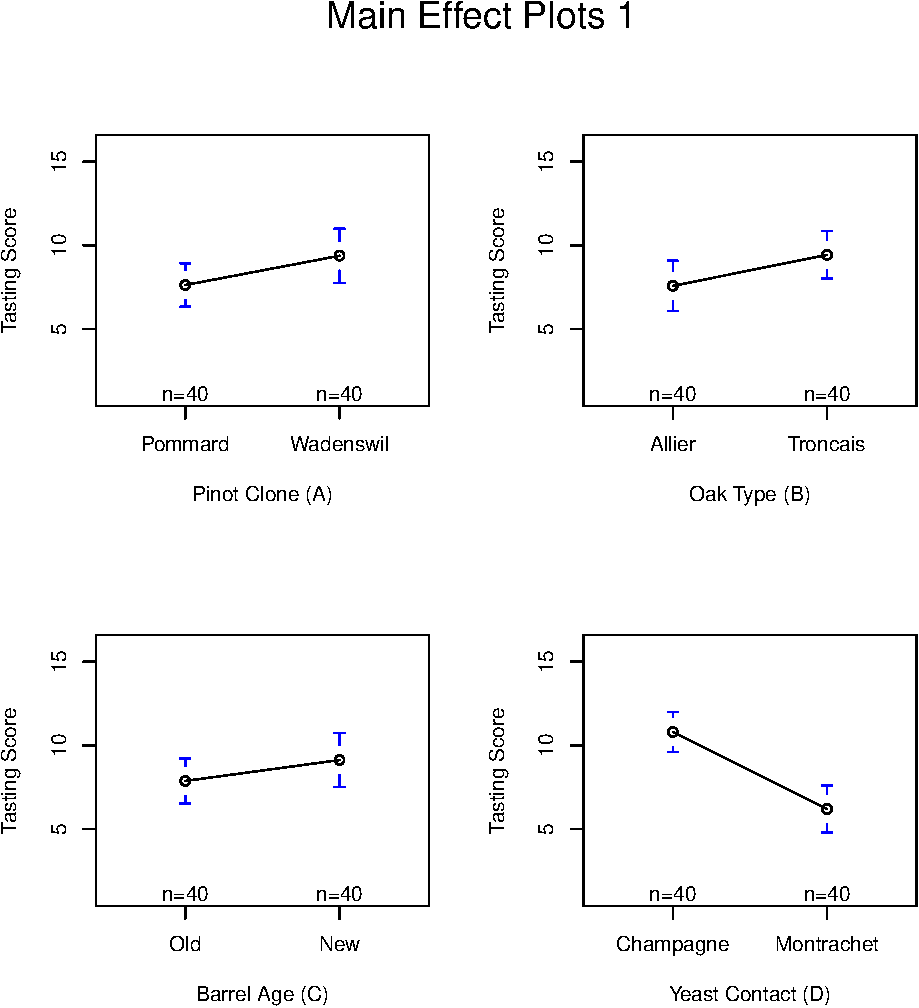
\includegraphics{wine_tasting_files/figure-latex/unnamed-chunk-7-1.pdf}

\begin{Shaded}
\begin{Highlighting}[]
\KeywordTok{plotmeans}\NormalTok{(}\DataTypeTok{formula =}\NormalTok{ y}\OperatorTok{~}\NormalTok{E, }\DataTypeTok{ylab =} \StringTok{"Tasting Score"}\NormalTok{, }\DataTypeTok{xlab =} \StringTok{"Stems (E)"}\NormalTok{, }\DataTypeTok{ylim =} \KeywordTok{c}\NormalTok{(}\DecValTok{1}\NormalTok{, }\DecValTok{16}\NormalTok{), }\DataTypeTok{data =}\NormalTok{ data, }\DataTypeTok{xaxt =} \StringTok{"n"}\NormalTok{)}
\KeywordTok{axis}\NormalTok{(}\DataTypeTok{side =} \DecValTok{1}\NormalTok{, }\DataTypeTok{at =} \KeywordTok{c}\NormalTok{(}\DecValTok{1}\NormalTok{,}\DecValTok{2}\NormalTok{), }\DataTypeTok{labels =} \KeywordTok{c}\NormalTok{(}\StringTok{"None"}\NormalTok{, }\StringTok{"All"}\NormalTok{))}
\KeywordTok{plotmeans}\NormalTok{(}\DataTypeTok{formula =}\NormalTok{ y}\OperatorTok{~}\NormalTok{F, }\DataTypeTok{ylab =} \StringTok{"Tasting Score"}\NormalTok{, }\DataTypeTok{xlab =} \StringTok{"Barrel Toast (F)"}\NormalTok{, }\DataTypeTok{ylim =} \KeywordTok{c}\NormalTok{(}\DecValTok{1}\NormalTok{, }\DecValTok{16}\NormalTok{), }\DataTypeTok{data =}\NormalTok{ data, }\DataTypeTok{xaxt =} \StringTok{"n"}\NormalTok{)}
\KeywordTok{axis}\NormalTok{(}\DataTypeTok{side =} \DecValTok{1}\NormalTok{, }\DataTypeTok{at =} \KeywordTok{c}\NormalTok{(}\DecValTok{1}\NormalTok{,}\DecValTok{2}\NormalTok{), }\DataTypeTok{labels =} \KeywordTok{c}\NormalTok{(}\StringTok{"Light"}\NormalTok{, }\StringTok{"Medium"}\NormalTok{))}
\KeywordTok{plotmeans}\NormalTok{(}\DataTypeTok{formula =}\NormalTok{ y}\OperatorTok{~}\NormalTok{G, }\DataTypeTok{ylab =} \StringTok{"Tasting Score"}\NormalTok{, }\DataTypeTok{xlab =} \StringTok{"Whole Cluster (G)"}\NormalTok{, }\DataTypeTok{ylim =} \KeywordTok{c}\NormalTok{(}\DecValTok{1}\NormalTok{, }\DecValTok{16}\NormalTok{), }\DataTypeTok{data =}\NormalTok{ data, }\DataTypeTok{xaxt =} \StringTok{"n"}\NormalTok{)}
\KeywordTok{axis}\NormalTok{(}\DataTypeTok{side =} \DecValTok{1}\NormalTok{, }\DataTypeTok{at =} \KeywordTok{c}\NormalTok{(}\DecValTok{1}\NormalTok{,}\DecValTok{2}\NormalTok{), }\DataTypeTok{labels =} \KeywordTok{c}\NormalTok{(}\StringTok{"None"}\NormalTok{, }\StringTok{"10%"}\NormalTok{))}
\KeywordTok{plotmeans}\NormalTok{(}\DataTypeTok{formula =}\NormalTok{ y}\OperatorTok{~}\NormalTok{H, }\DataTypeTok{ylab =} \StringTok{"Tasting Score"}\NormalTok{, }\DataTypeTok{xlab =} \StringTok{"Fermentation Temp (H)"}\NormalTok{, }\DataTypeTok{ylim =} \KeywordTok{c}\NormalTok{(}\DecValTok{1}\NormalTok{, }\DecValTok{16}\NormalTok{), }\DataTypeTok{data =}\NormalTok{ data, }\DataTypeTok{xaxt =} \StringTok{"n"}\NormalTok{)}
\KeywordTok{axis}\NormalTok{(}\DataTypeTok{side =} \DecValTok{1}\NormalTok{, }\DataTypeTok{at =} \KeywordTok{c}\NormalTok{(}\DecValTok{1}\NormalTok{,}\DecValTok{2}\NormalTok{), }\DataTypeTok{labels =} \KeywordTok{c}\NormalTok{(}\StringTok{"Low"}\NormalTok{, }\StringTok{"High"}\NormalTok{))}
\KeywordTok{mtext}\NormalTok{(}\StringTok{"Main Effect Plots 2"}\NormalTok{, }\DataTypeTok{outer =} \OtherTok{TRUE}\NormalTok{, }\DataTypeTok{cex =} \FloatTok{1.5}\NormalTok{)}
\end{Highlighting}
\end{Shaded}

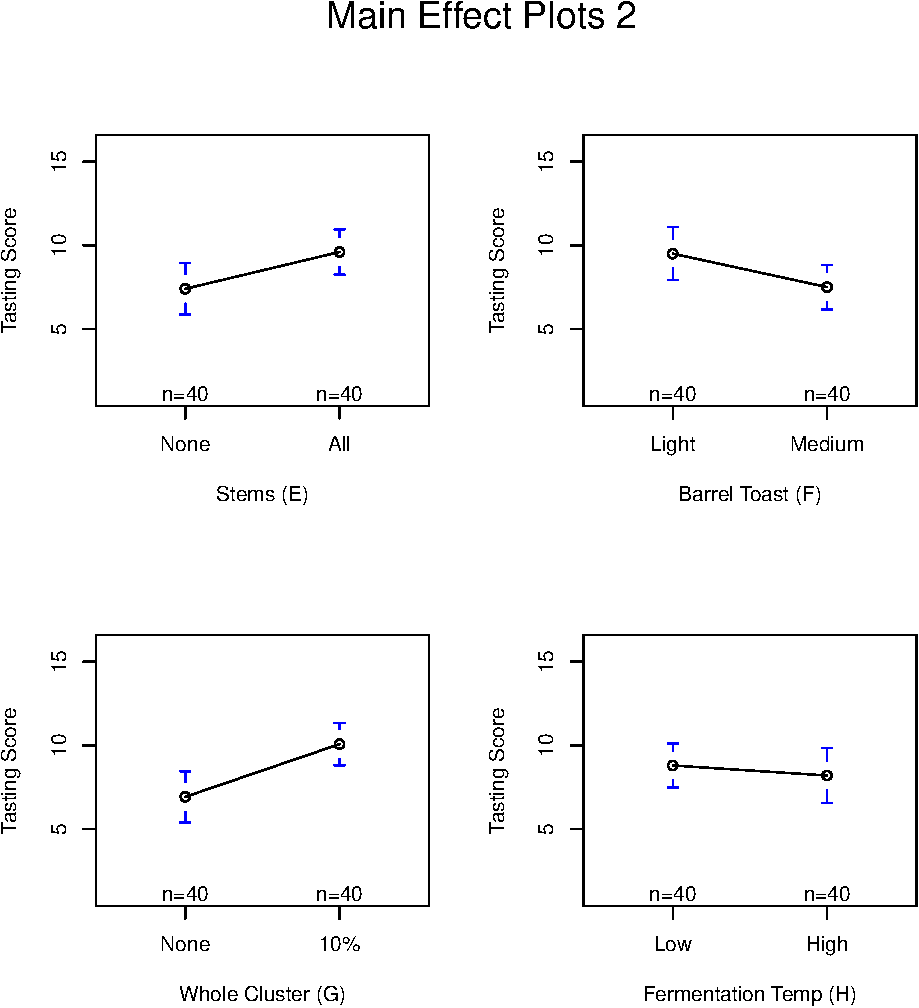
\includegraphics{wine_tasting_files/figure-latex/unnamed-chunk-7-2.pdf}

Notes: It is clear that yeast type (D) and the amount of whole clusters
(G) used during fermentation are most important, with no whole clusters
and Montrachet yeast producing a better tasting wine. Although not
significant, medium barrel toast (F) and no stems (E) seem to correspond
to a better tasting Pinot Noir.

\newpage

\begin{Shaded}
\begin{Highlighting}[]
\CommentTok{## Interaction Plots}
\KeywordTok{par}\NormalTok{(}\DataTypeTok{mfrow=}\KeywordTok{c}\NormalTok{(}\DecValTok{1}\NormalTok{,}\DecValTok{3}\NormalTok{), }\DataTypeTok{oma =} \KeywordTok{c}\NormalTok{(}\DecValTok{0}\NormalTok{,}\DecValTok{0}\NormalTok{,}\DecValTok{2}\NormalTok{,}\DecValTok{0}\NormalTok{))}
\CommentTok{# par(mfrow=c(1,3), oma = c(0,0,0,0))}
\KeywordTok{interaction.plot}\NormalTok{(D, F, y, }\DataTypeTok{ylab =} \StringTok{"Mean Response Rate"}\NormalTok{, }\DataTypeTok{xlab =} \StringTok{"Yeast Type (D)"}\NormalTok{, }\DataTypeTok{main =} \StringTok{""}\NormalTok{, }\DataTypeTok{ylim =} \KeywordTok{c}\NormalTok{(}\DecValTok{1}\NormalTok{, }\DecValTok{16}\NormalTok{), }\DataTypeTok{legend =} \OtherTok{FALSE}\NormalTok{)}
\KeywordTok{points}\NormalTok{(}\DataTypeTok{x =} \KeywordTok{c}\NormalTok{(}\DecValTok{1}\NormalTok{,}\DecValTok{1}\NormalTok{), }\DataTypeTok{y =} \KeywordTok{c}\NormalTok{(}\KeywordTok{mean}\NormalTok{(data[data}\OperatorTok{$}\NormalTok{D}\OperatorTok{==-}\DecValTok{1} \OperatorTok{&}\StringTok{ }\NormalTok{data}\OperatorTok{$}\NormalTok{F}\OperatorTok{==-}\DecValTok{1}\NormalTok{,]}\OperatorTok{$}\NormalTok{y),}\KeywordTok{mean}\NormalTok{(data[data}\OperatorTok{$}\NormalTok{D}\OperatorTok{==-}\DecValTok{1} \OperatorTok{&}\StringTok{ }\NormalTok{data}\OperatorTok{$}\NormalTok{F}\OperatorTok{==}\DecValTok{1}\NormalTok{,]}\OperatorTok{$}\NormalTok{y)), }\DataTypeTok{pch =} \DecValTok{1}\NormalTok{)}
\KeywordTok{points}\NormalTok{(}\DataTypeTok{x =} \KeywordTok{c}\NormalTok{(}\DecValTok{2}\NormalTok{,}\DecValTok{2}\NormalTok{), }\DataTypeTok{y =} \KeywordTok{c}\NormalTok{(}\KeywordTok{mean}\NormalTok{(data[data}\OperatorTok{$}\NormalTok{D}\OperatorTok{==}\DecValTok{1} \OperatorTok{&}\StringTok{ }\NormalTok{data}\OperatorTok{$}\NormalTok{F}\OperatorTok{==-}\DecValTok{1}\NormalTok{,]}\OperatorTok{$}\NormalTok{y),}\KeywordTok{mean}\NormalTok{(data[data}\OperatorTok{$}\NormalTok{D}\OperatorTok{==}\DecValTok{1} \OperatorTok{&}\StringTok{ }\NormalTok{data}\OperatorTok{$}\NormalTok{F}\OperatorTok{==}\DecValTok{1}\NormalTok{,]}\OperatorTok{$}\NormalTok{y)), }\DataTypeTok{pch =} \DecValTok{1}\NormalTok{)}
\KeywordTok{legend}\NormalTok{(}\StringTok{"bottomleft"}\NormalTok{, }\DataTypeTok{legend =} \KeywordTok{c}\NormalTok{(}\StringTok{"Toast (F)"}\NormalTok{,}\StringTok{"Medium"}\NormalTok{, }\StringTok{"Light"}\NormalTok{), }\DataTypeTok{lty =} \KeywordTok{c}\NormalTok{(}\DecValTok{1}\NormalTok{,}\DecValTok{1}\NormalTok{,}\DecValTok{2}\NormalTok{), }\DataTypeTok{col=}\KeywordTok{c}\NormalTok{(}\StringTok{"white"}\NormalTok{, }\StringTok{"black"}\NormalTok{, }\StringTok{"black"}\NormalTok{), }\DataTypeTok{cex =} \FloatTok{0.75}\NormalTok{)}
\KeywordTok{interaction.plot}\NormalTok{(F, G, y, }\DataTypeTok{ylab =} \StringTok{"Mean Response Rate"}\NormalTok{, }\DataTypeTok{xlab =} \StringTok{"Barrel Toast (F)"}\NormalTok{, }\DataTypeTok{main =} \StringTok{""}\NormalTok{, }\DataTypeTok{ylim =} \KeywordTok{c}\NormalTok{(}\DecValTok{1}\NormalTok{, }\DecValTok{16}\NormalTok{), }\DataTypeTok{legend =} \OtherTok{FALSE}\NormalTok{)}
\KeywordTok{points}\NormalTok{(}\DataTypeTok{x =} \KeywordTok{c}\NormalTok{(}\DecValTok{1}\NormalTok{,}\DecValTok{1}\NormalTok{), }\DataTypeTok{y =} \KeywordTok{c}\NormalTok{(}\KeywordTok{mean}\NormalTok{(data[data}\OperatorTok{$}\NormalTok{F}\OperatorTok{==-}\DecValTok{1} \OperatorTok{&}\StringTok{ }\NormalTok{data}\OperatorTok{$}\NormalTok{G}\OperatorTok{==-}\DecValTok{1}\NormalTok{,]}\OperatorTok{$}\NormalTok{y),}\KeywordTok{mean}\NormalTok{(data[data}\OperatorTok{$}\NormalTok{F}\OperatorTok{==-}\DecValTok{1} \OperatorTok{&}\StringTok{ }\NormalTok{data}\OperatorTok{$}\NormalTok{G}\OperatorTok{==}\DecValTok{1}\NormalTok{,]}\OperatorTok{$}\NormalTok{y)), }\DataTypeTok{pch =} \DecValTok{1}\NormalTok{)}
\KeywordTok{points}\NormalTok{(}\DataTypeTok{x =} \KeywordTok{c}\NormalTok{(}\DecValTok{2}\NormalTok{,}\DecValTok{2}\NormalTok{), }\DataTypeTok{y =} \KeywordTok{c}\NormalTok{(}\KeywordTok{mean}\NormalTok{(data[data}\OperatorTok{$}\NormalTok{F}\OperatorTok{==}\DecValTok{1} \OperatorTok{&}\StringTok{ }\NormalTok{data}\OperatorTok{$}\NormalTok{G}\OperatorTok{==-}\DecValTok{1}\NormalTok{,]}\OperatorTok{$}\NormalTok{y),}\KeywordTok{mean}\NormalTok{(data[data}\OperatorTok{$}\NormalTok{F}\OperatorTok{==}\DecValTok{1} \OperatorTok{&}\StringTok{ }\NormalTok{data}\OperatorTok{$}\NormalTok{G}\OperatorTok{==}\DecValTok{1}\NormalTok{,]}\OperatorTok{$}\NormalTok{y)), }\DataTypeTok{pch =} \DecValTok{1}\NormalTok{)}
\KeywordTok{legend}\NormalTok{(}\StringTok{"bottomleft"}\NormalTok{, }\DataTypeTok{legend =} \KeywordTok{c}\NormalTok{(}\StringTok{"Whole Cluster (G)"}\NormalTok{,}\StringTok{"10%"}\NormalTok{, }\StringTok{"None"}\NormalTok{), }\DataTypeTok{lty =} \KeywordTok{c}\NormalTok{(}\DecValTok{1}\NormalTok{,}\DecValTok{1}\NormalTok{,}\DecValTok{2}\NormalTok{), }\DataTypeTok{col=}\KeywordTok{c}\NormalTok{(}\StringTok{"white"}\NormalTok{, }\StringTok{"black"}\NormalTok{, }\StringTok{"black"}\NormalTok{), }\DataTypeTok{cex =} \FloatTok{0.75}\NormalTok{)}
\KeywordTok{interaction.plot}\NormalTok{(E, G, y, }\DataTypeTok{ylab =} \StringTok{"Mean Response Rate"}\NormalTok{, }\DataTypeTok{xlab =} \StringTok{"Stems (E)"}\NormalTok{, }\DataTypeTok{main =} \StringTok{""}\NormalTok{, }\DataTypeTok{ylim =} \KeywordTok{c}\NormalTok{(}\DecValTok{1}\NormalTok{, }\DecValTok{16}\NormalTok{), }\DataTypeTok{legend =} \OtherTok{FALSE}\NormalTok{)}
\KeywordTok{points}\NormalTok{(}\DataTypeTok{x =} \KeywordTok{c}\NormalTok{(}\DecValTok{1}\NormalTok{,}\DecValTok{1}\NormalTok{), }\DataTypeTok{y =} \KeywordTok{c}\NormalTok{(}\KeywordTok{mean}\NormalTok{(data[data}\OperatorTok{$}\NormalTok{E}\OperatorTok{==-}\DecValTok{1} \OperatorTok{&}\StringTok{ }\NormalTok{data}\OperatorTok{$}\NormalTok{G}\OperatorTok{==-}\DecValTok{1}\NormalTok{,]}\OperatorTok{$}\NormalTok{y),}\KeywordTok{mean}\NormalTok{(data[data}\OperatorTok{$}\NormalTok{E}\OperatorTok{==-}\DecValTok{1} \OperatorTok{&}\StringTok{ }\NormalTok{data}\OperatorTok{$}\NormalTok{G}\OperatorTok{==}\DecValTok{1}\NormalTok{,]}\OperatorTok{$}\NormalTok{y)), }\DataTypeTok{pch =} \DecValTok{1}\NormalTok{)}
\KeywordTok{points}\NormalTok{(}\DataTypeTok{x =} \KeywordTok{c}\NormalTok{(}\DecValTok{2}\NormalTok{,}\DecValTok{2}\NormalTok{), }\DataTypeTok{y =} \KeywordTok{c}\NormalTok{(}\KeywordTok{mean}\NormalTok{(data[data}\OperatorTok{$}\NormalTok{E}\OperatorTok{==}\DecValTok{1} \OperatorTok{&}\StringTok{ }\NormalTok{data}\OperatorTok{$}\NormalTok{G}\OperatorTok{==-}\DecValTok{1}\NormalTok{,]}\OperatorTok{$}\NormalTok{y),}\KeywordTok{mean}\NormalTok{(data[data}\OperatorTok{$}\NormalTok{E}\OperatorTok{==}\DecValTok{1} \OperatorTok{&}\StringTok{ }\NormalTok{data}\OperatorTok{$}\NormalTok{G}\OperatorTok{==}\DecValTok{1}\NormalTok{,]}\OperatorTok{$}\NormalTok{y)), }\DataTypeTok{pch =} \DecValTok{1}\NormalTok{)}
\KeywordTok{legend}\NormalTok{(}\StringTok{"bottomleft"}\NormalTok{, }\DataTypeTok{legend =} \KeywordTok{c}\NormalTok{(}\StringTok{"Whole Cluster (G)"}\NormalTok{,}\StringTok{"10%"}\NormalTok{, }\StringTok{"None"}\NormalTok{), }\DataTypeTok{lty =} \KeywordTok{c}\NormalTok{(}\DecValTok{1}\NormalTok{,}\DecValTok{1}\NormalTok{,}\DecValTok{2}\NormalTok{), }\DataTypeTok{col=}\KeywordTok{c}\NormalTok{(}\StringTok{"white"}\NormalTok{, }\StringTok{"black"}\NormalTok{, }\StringTok{"black"}\NormalTok{), }\DataTypeTok{cex =} \FloatTok{0.75}\NormalTok{)}
\KeywordTok{mtext}\NormalTok{(}\StringTok{"Interaction Plots"}\NormalTok{, }\DataTypeTok{outer =} \OtherTok{TRUE}\NormalTok{, }\DataTypeTok{cex =} \FloatTok{1.5}\NormalTok{)}
\end{Highlighting}
\end{Shaded}

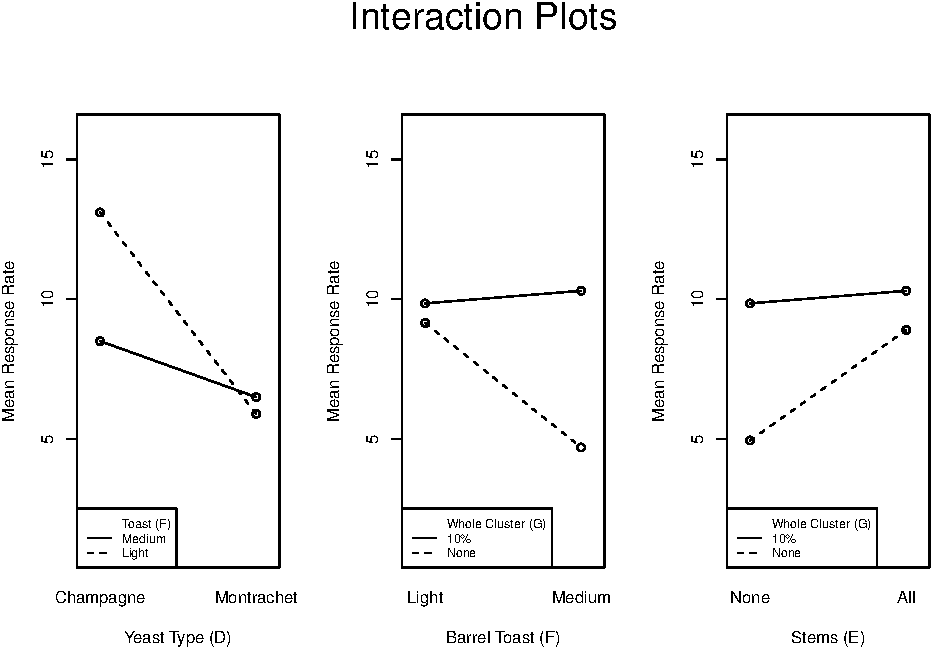
\includegraphics{wine_tasting_files/figure-latex/unnamed-chunk-8-1.pdf}

Notes: If yeast type is Montrachet, barrel toast doesn't matter much,
but if yeast type is Champagne, a medium barrell toast is best. And if
barrel toast is chosen to be medium, then not including any
whole-clusters is best. If using none of the stems, then don't use whole
clusters.

Conclusions: This study was able to identify a small number of important
factors and interactions that influence a Pinot Noir's flavor. Perhaps
importantly, it has identified which factors do not have a significant
influence. In line with the philosophy of sequential experimentation,
this information can then be exploited in future studies.


\end{document}
